
\let\negmedspace\undefined
\let\negthickspace\undefined
\documentclass[journal]{IEEEtran}
\usepackage[a5paper, margin=10mm, onecolumn]{geometry}
%\usepackage{lmodern} % Ensure lmodern is loaded for pdflatex
\usepackage{tfrupee} % Include tfrupee package
\setlength{\headheight}{1cm} % Set the height of the header box
\setlength{\headsep}{0mm}     % Set the distance between the header box and the top of the text
\usepackage{gvv-book}
\usepackage{gvv}
\usepackage{cite}
\usepackage{amsmath,amssymb,amsfonts,amsthm}
\usepackage{algorithmic}
\usepackage{graphicx}
\usepackage{textcomp}
\usepackage{xcolor}
\usepackage{txfonts}
\usepackage{listings}
\usepackage{enumitem}
\usepackage{mathtools}
\usepackage{gensymb}
\usepackage{comment}
\usepackage[breaklinks=true]{hyperref}
\usepackage{tkz-euclide} 
\usepackage{listings}
% \usepackage{gvv}                                        
\def\inputGnumericTable{}                                 
\usepackage[latin1]{inputenc}                                
\usepackage{color}                                            
\usepackage{array}                                            
\usepackage{longtable}                                       
\usepackage{calc}                                             
\usepackage{multirow}                                         
\usepackage{hhline}                                           
\usepackage{ifthen}                                           
\usepackage{lscape}
\renewcommand{\thefigure}{\theenumi}
\renewcommand{\thetable}{\theenumi}
\setlength{\intextsep}{10pt} % Space between text and floats
\numberwithin{equation}{enumi}
\numberwithin{figure}{enumi}
\renewcommand{\thetable}{\theenumi}
\begin{document}
\bibliographystyle{IEEEtran}
\title{Question 4-4.4-35}
\author{EE24BTECH11015 - Dhawal}
% \maketitle
% \newpage
% \bigskip
{\let\newpage\relax\maketitle}
\begin{enumerate}
\item Find the value of x such that the four points $\vec{A}  \brak{x , 5 , -1}, \vec{B} \brak{3 , 2 , 1},\vec{C} 
\brak{4 , 5 , 5} \text{ and } \vec{D}
\brak{4 , 2 , -2}$ are coplanar.

\end{enumerate}

\begin{table}[h!]    
  \centering
  
\begin{tabular}[12pt]{ |c| c| c|}
    \hline
    \textbf{Variable} & \textbf{Description} & \textbf{Values} \\ 
    \hline
    AB & Length & 6 cm \\
    \hline
    BC & Length & 8 cm \\
    \hline
    $\angle ABC$ & Angle & \ang{60}\\
    \hline 
    $\vec{A}$ & Point & $(6,0)$ \\
    \hline
    $\vec{B}$ & Origin & $(0,0)$ \\
    \hline
    $\vec{C}$ & To find & ? \\
    \hline
    \end{tabular}


  \caption{Variables given}
  \label{tab 1.4.9.2}
\end{table}
Solution:\\
Matrix with all 3 vectors: 
\begin{align}
       {\myvec{DC && BC&& AC}}^T
\end{align}
If these points are coplaner, the matrix should have rank less than 3,
\begin{align}
	\myvec{0&&3&&7\\1&&3&&4\\4-x&&0&&6}
\end{align}
$R_2 \rightarrow R_2-R_1$
\begin{align}
	\myvec{0&&3&&7\\1&&0&&-3\\4-x&&0&&6}
\end{align}
$R_3 \rightarrow R_3+2R_2$
\begin{align}
	\myvec{0&&3&&7\\1&&0&&-3\\6-x&&0&&0}
\end{align}
The last row should be zero,
\begin{align}
	6-x=0 \rightarrow x=6
\end{align}





Plot:
\begin{figure}[h!]
   \centering
   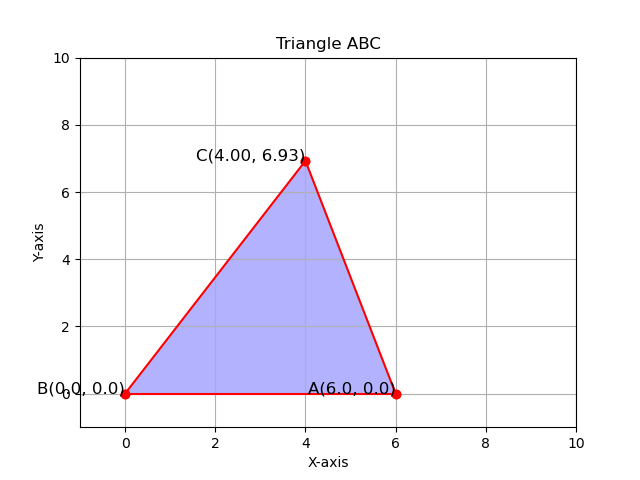
\includegraphics[width=0.9\linewidth]{Figure_1.png}
	\caption{$\Delta ABC$ }
   \label{stemplot}
\end{figure}


\end{document}

